\section{Caractérisation des architectures}\label{sec:caracterisation}


\textbf{TODO}
- lecture thèse - 1 Décomposition automatique des programmes parallèles pour l’optimisation et la prédiction de performance. Mihail Popov\\




%%%%%%%%%%%%%%%%%%%%%%%%%%%%%%%%%
\subsection{Benchmarks}
%%%%%%%%%%%%%%%%%%%%%%%%%%%%%%%%%

En informatique, un benchmark est un code, ou un ensemble de code, permettant de mesurer la performance d'une solution et d'en vérifier ses fonctionnalités. Les benchmarks peuvent être utilisés pour plusieurs raisons, énumérée dans le paragraphe suivant. 

% UTILITE
\paragraph{Utilité des benchmarks.}
Dans le domaine du HPC, les benchmarks sont utilisés pour raisons différentes. 
    
    De nombreuses architectures sont présentés chaque années, avec chacune des caractéristiques différentes. Pour connaître leur potentiel, des codes de références sont utilisés pour apprécier leur performances pour un certain types d'application. 
    
    Les benchmarks peuvent aussi être utilisés lors de la phase de conception d'une architecture. Cela permet d'estimer la futur performance d'un matériel avant qu'il ne soit produit (grâce à des simulateurs par exemple). Les benchmarks utilisés peuvent avoir les mêmes profils que les applications qui seront réellement exécutées sur le supercalculateur en production. Cela permet à l'industriel qui le produit de la placer sur des domaines sur lesquels il performe particulièrement.
     
    
    Utiliser un benchmark évite à l'acheteur de fournir des codes et des données (souvent sensibles) pour la conception d'une plate-forme. En utilisant un benchmark, il est facile pour un concepteur de cluster de tester différentes configuration sur des processeurs différents, avec des tailles de mémoires plus ou moins grandes et des réseaux de vitesses différentes. 
    Les codes de benchmark sont plus la majorité en version libre de droit. Cela permet leur large utilisation et permet de comparer la performance de différentes plate-formes. Le TOP500 réalisé grâce au benchmark HPL en est un exemple.
     
    
    Aussi, les centres de données sont des zones très sensibles. Il arrive que les ingénieurs ayant construit le supercalculateur n'y ai même plus accès une fois ce dernier installé. En utilisant des benchmarks libre de droit, l'utilisateur peur l'exécuter et renvoyer le profil extrait pour permettre aux architectes d'en comprendre les performances. L'utilisation de benchmark dont le code est souvent beaucoup plus simple que celui des applications réelles permet de rapidement identifier des problèmes de performances. 
    
    La complexité des architectures rend difficile la prédiction de la performance d'une plate-forme par la simple lecture de ses caractéristiques techniques ($PERFORMANCE_{crête}$). Il est donc nécessaire d'utiliser une application pour en mesurer la performance maximale atteignable ($PERFORMANCE_{max}$). Le classement du TOp500 fournit ces informations et on constate de grand écart entre ces deux performance pouvant être de plus de 50\%. Le code des benchmarks étant plus simple que celui des applications, un utilisateur voulant atteindre la performance maximale avec son application pourra regarder comment le benchmark a été codé. 


\paragraph{Trois types de benchmarks} Il existe différents types de benchmarks qui peuvent être classés en trois familles \cite{Staelin2004}: les benchmarks, les benchmarks noyaux et les micro-benchmarks.
    
    Les benchmark sont des applications complètes exécutant différent types d'instructions: calculs, transferts mémoire, réseaux... Il peut aussi arriver que des applications réelles soient finalement utilisées comme programme de benchmark tel que BSMBnech \cite{HPC:bsmbench} utilisé pour réaliser des motifs de calculs similaires à ceux de en théorie de jauge sur réseau (physique des particules).
    
    La deuxième famille de benchmarks regroupe les benchmarks noyaux. Ces codes sont généralement extraits d'un application et sont donc plus petits. Les deux benchmark les plus connus sont HPL \cite{HPC:hpl} et STREAM \cite{HPC:stream}. Le benchmark STREAM conciste en l'exécution de quatre fonctions différentes très utilisés dans les application HPC. A l'origine utilisée pour étudier les différences de performances entre deux architectures pour exécuter des applications pour la modélisation du climat, ce code est aujourd'hui très utiliser pour mesurer la bande passante mémoire atteignable sur un bus mémoire. 
   
    Enfin, les micro-benchmark sont des benchmark noyaux qui permettent un d’isoler la partie de l’architecture à stresser. Plus simples, ils permettent de tirer des conclusion sur la performance du matériel. Cela permet d’être sur que l’on mesure bien ce que l’on souhaite et que la performance mesurée n’est pas influé par une autre partie.
    Par exemple, lmbench \cite{HPC:lmbench} est une suite de benchmarks portables utilisés pour mesurer des caractéristiques importantes de la mémoire telles que la bande passante, la latence mémoire et les performances des différents niveaux de cache.
    On peut également citer les travaux \cite{Saavedra1995, gonzalez2010servet} pour la caractérisation des différents niveaux de la hiérarchie mémoire. Les informations récupérées permettent ensuite d'implémenter des optimisations telles que le le \textit{loop tiling} pour s'adapter parfaitement aux différents niveaux de caches.



\paragraph{Construction d'un benchmark} Pour construire un benchmark, deux méthodes peuvent être utilsées. 
    La première est de l'écrire en s'inspirant d'une application réelle ou en implémentant des fonctions pour \textit{stresser} certaines parties de la plate-forme.
    La deuxième méthode est de générer un code de benchmark grâce à un premier code générateur. La génération a l'avantage de faciliter le test de plusieurs configurations différentes en faisant varier les paramètres d'entrée, la taille des jeux de données, ou encore l'algorithme utilisé pour résoudre une tâche. Ainsi, le logiciel de GeneNetWeaver \cite{schaffter2011genenetweaver} peut être utilisé pour générer dynamiquement des modèles génétiques pouvant ensuite eux même être utilisés comme benchmark. Le Benchmark Generator (BM) \cite{younes2003benchmark} peut lui être utilisé pour résoudre dynamiquent le problème du \textit{voyageur de commerce}.


\subsubsection{Les benchmark de processeur}
%%%%%%%%%%%%%%%%%%%%%%%%%%%%%%%%%


\paragraph{HGEMM}






\paragraph{HPL} Les premières versions du benchmark remonte aux années 1979. Le benchmark LINPACK était alors utilisé pour estimer le temps de résolution d'un problème d'algèbre. Ce programme utilisait alors une bibliothèque mathématiques du même nom \textit{LINPACK}. Son utilisation comme benchmark est plus un accident qu'une réelle volonté. L'annexe B du manuel de l'utilisateur proposait aux utilisateeurs d'estimer les temps de résolution de leur problème en fonction de la machine utilisée. Pour pouvoir être utilisé sur les supercalculateurs, le benchmark à été parallélisé, changeant ainsi de nom en Highly Parallel Computing Benchmark ou HPLinpack ou encore HPL.  Le benchmark HPL est utilisé pour construire le  classement du \textit{Top500} \cite{HPC:top500}. Il est utilisé pour mesurer le nombre maximum d'opération à virgule flottantes par seconde (FLOPS) qu'un superordinateur est capable de fournir en résolvant un système linéaire d'équations utilisant la décomposition LU. Ainsi, avant d'être un benchmark de processeur, c'est un benchmark de librairie DGEMM (Intel MKL, netlib, GotoBLAS). La force de ce benchmark est de n'avoir qu'un résultat (soit la sommation des puissances de calculs de chaque coeur utilisé). Il est donc très facile de comparer deux clusters. Bien que mondialement utilisé, le HPL à un principale défaut qui est d'estimer la performance d'une plate-forme en ne mesurant que sa capacité de calcul. Cependant, comme nous l'avons montré précédemment, la performance de la majorité des applications est limitée par la performance de la bande passante. La mesure du HPL n'est donc pas la plus représentative de la puissance d'un supercalculateur atteignables par des applications réelles. 




\paragraph{High Performance Conjugate Gradient (HPCG) \cite{Dongarra2013}} 
Admettant la faiblesse du benchmark HPL son concepteur, Jack Dongarra, se mis à la recherche d'un ou d'un ensemble de benchmark permettant de mieux caractériser ces plate-formes. Avec Michael Heroux et Piotr Luszczek ils présenteront alors en 2015 le benchmark HPCG (high performance conjugate gradient). HPCG permet de couvrir de nombreux motifs de communication (globale et voisinage) et de calculs  (mis-à-jour de vecteur, multiplication de matrices creuses). 
Le premier pré-requis étaient alors de pouvoir produire, grâce à ce nouveau benchmark, un classement des supercalculateurs représentatif de leur performance pour exécuter des applications réelles. Le deuxième pré-requis fait suite à la crainte de voir la conception des processeurs adapté à leur performance pour HPL \cite{Dongarra2013}. Ainsi, HPCG utilise une métric qui poussera les concepteurs de processeurs à améliorer leurs matériels pouvant profiter aux applications réelles. Là où HPL ne fournit qu'un seul résultat par exécution, HPCG en présente 128. Le classement du Top500 est aujourd'hui publié avec les valeurs obtenues par HPL et par HPCG\footnote{classement HPCG: \url{https://www.top500.org/hpcg/lists/2018/06/}}. Bien que plus représentatif des applications réelles que le benchmark HPL, il ne couvre qu'un seul type d'application ayant un faible ratio d'accès mémoire par calcul effectué. Cependant, malgré la meilleur adéquation de HPCG pour caractériser les plate-formes, le benchmark HPL sera toujours utilisé. Principalement pour des raisons d'historiques, il permet de suivre l'évolution des architectures depuis plus de 25 ans. 





\paragraph{HPC Challenge (HPCC)} Cette suite de benchmark vient compléter le benchmark HPL avec des 6 codes dont certains réalisant des accès aux données permettant aussi de caractériser le système mémoire (voir \autoref{pic_bench_hpcc}). La suite de benchmark est ainsi composé de HPL, Stream, DGEMM, RandomAccess, b\_eff, PTRANS, FFT. Avec l'ajout de ces six autres codes, la suite HPCC est plus représentative des applications réelles Ces codes existaient avant la création de la suite HPCC. Le travail réalisé a permis de les regrouper dans une même suite, et de les améliorer avec des systèmes de vérifications et de rapport. Une fois compilé, un seul programme exécutable et généré permettant de faciliter son usage avec un gestionnaire de \textit{job}\footnote{\url{http://citeseerx.ist.psu.edu/viewdoc/download?doi=10.1.1.170.1239&rep=rep1&type=pdf}}. Un seul exécutable étant généré, l'environnement d'exécution est le même pour tous les benchmark de la suite (pas d'optimisaion de page large pour un seul benchmark de la suite). 

\begin{figure}
    \center
    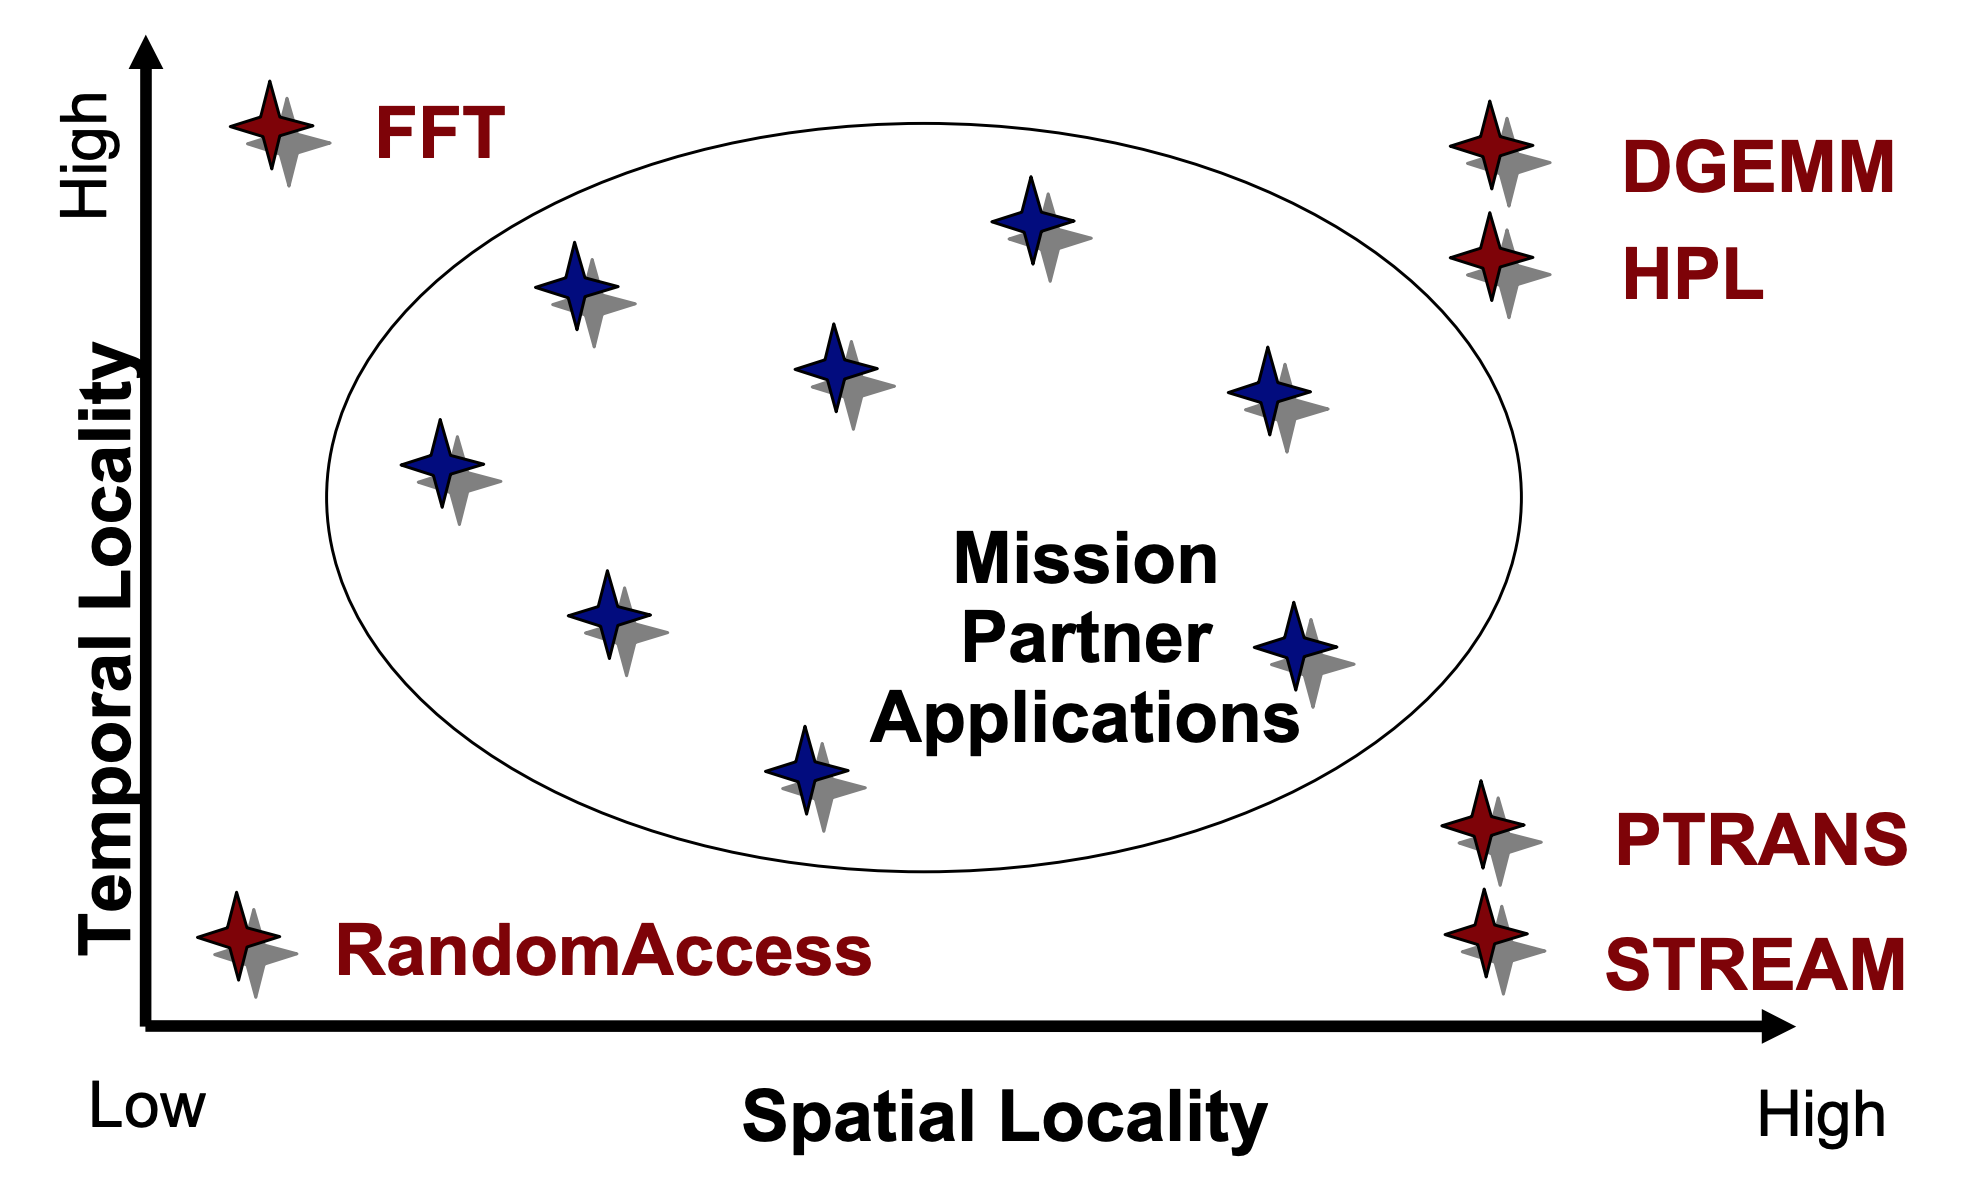
\includegraphics[width=10cm]{images/bench_hpcc.png}
    \caption{ La suite de benchmark HPCC utilise des codes utilisant des localités différentes permettant de mieux caractériser les architectures
    \label{pic_bench_hpcc}}
\end{figure}





\paragraph{NAS Parallel Benchmarks} Ce benchmark développé par la NASA est un ensemble de code permettant d'évaluer la performance de calculs d'un supercalculateur. Le code regroupe cinq kernels et trois petite application dérivé d'application du domaine de la mécanique des fluides. Bien que similaire à HPCG, la différence principale vient de l'initialisation des matrices utilisant une distribution uniforme des données dans chaque ligne. Ce manque de réalisme et la non utilisation de préconditionnement font du benchmark HPCG une meilleure alternative pour ce genre de tests. De plus, les imlémentations des benchmarks divergent entre chaque architecture rendant leur comparaison plus difficile.




\paragraph{SPEC CPU2017} Cette nouvelle génération de benchmark produite par SPEC (Standard Performance Evaluation Corporation) qui fait suite à la version précédente CPEC CPU2006. Ces deux initiatives ont permis de regrouper des applications réelles de tailles différentes mais donc les performances sont limités par la puissance de calcul de l'architecture. Les applications sélectionnés sont facilement portables. La première version contenait deux suites de benchmarks (CINT2006 et CFP2006à permettant demesurer et comparer les performances de calculs en utilisant des opérations entières ou à nombre flottant. L'objectif principale de ce ces codes était alors de caractériser les perofrmance du processeur, de la hiérachie mémoire et du compilateur. La version 2017 possède 43 benchmarks qui sont portées sur plusieurs architectures dont AMD64, Intel IA32, Power ISA ou SPARC. Les benchmarks sont organisés en quatre suites permetant de mesurer le débit et vitesse d'exécution d'opérations utilisant des nombres entiers ou flottant.  Les différents benchmarks ont un domaine d'application spécifique (compression vidéo, rendu 3D...) et peuvent être utilisé pour la conception de processeur optimisés pour ces charges de travail \cite{Panda2018}. Malheureusement le prix de ces benchmarks avoisine les 1000\$. Cependant les nombreux résultats, libres de droits, sont publiés leur site internet. 

\paragraph{SHOC \cite{danalis2010scalable}.} Les plate-formes HPC modernes deviennent toujours plus hétérogènes avec l'utilisation d'accélérateurs comme les GPU ou les DSP. Suite à ce constat, la suite de benchmark Scalable HeterOgeneous Computing (SHOC) a été élaborée pour permettre l'évaluation de la performance et de la montée en charge de tels systèmes. La suite est composée de micro-benchmark et de kernel-benchmark permettant d'évaluer précisément une architecture mais aussi celle d'une plate-forme regroupant plusieurs serveurs grâce à une implémentation MPI. Les codes utilise OpenCL et CUDA pour permettre une large utilisation. Une partie des codes est utiliser pour stresser l'achitecture et identifier des problèmes matériels pouvant impacter la performance: mémoire défaillante ou un mauvais refroidissement. L'autre partie des codes est utilisé pour mesurer la performance de l'architecture grâce à des applications proches de celles utilisés en production. Le code source de la suite de benchmarks est disponible en ligne \footnote{\url{https://github.com/vetter/shoc/wiki}}.


\paragraph{lmbench ici}
In lmbench, McVoy and Staelin replaced array access with
a linked list traversal to allow indirect and randomized access
patterns [7]. This advance was necessitated by improvements
in hardware prefetching

\paragraph{X-Ray \cite{Yotov2004}} Pour aider les programmeurs à écrire de nouveaux benchmarks permettant de mesurer certains paramètres matériel l'outil X-Ray a été mis au point. X-Ray est un framework permettant l'automatisation du développement de benchmark. L'outil est capable de générer plusieurs benchmark dynamiquement en tenant compte de l'exécution des premières versions. Si un benchmark a besoin de connaitre la latence mémoire d'un niveau de cache, X-Ray exécutera alors le benchmark permettant de le calculer avant. X-Ray peut par exemple calculer la fréquence du processeur en ajoutant quatre nombres entiers avec des dépendances pour éviter les optimisations des processeurs superscalaires. Des benchmarks sont aussi disponible pour caractériser la hiérarchie mémoire (associativé, taille des blocs, capacité, latence). Les résultats présentés sont annoncés plus précis que ceux donné par les autres outils de l'état de l'art. Différents tests ont été réalisés sur des ordinateur personnel, des serveurs ou encore des systèmes embarqués. Malheureusement le code n'est plus disponible pour être testé. 

\begin{figure}
    \center
    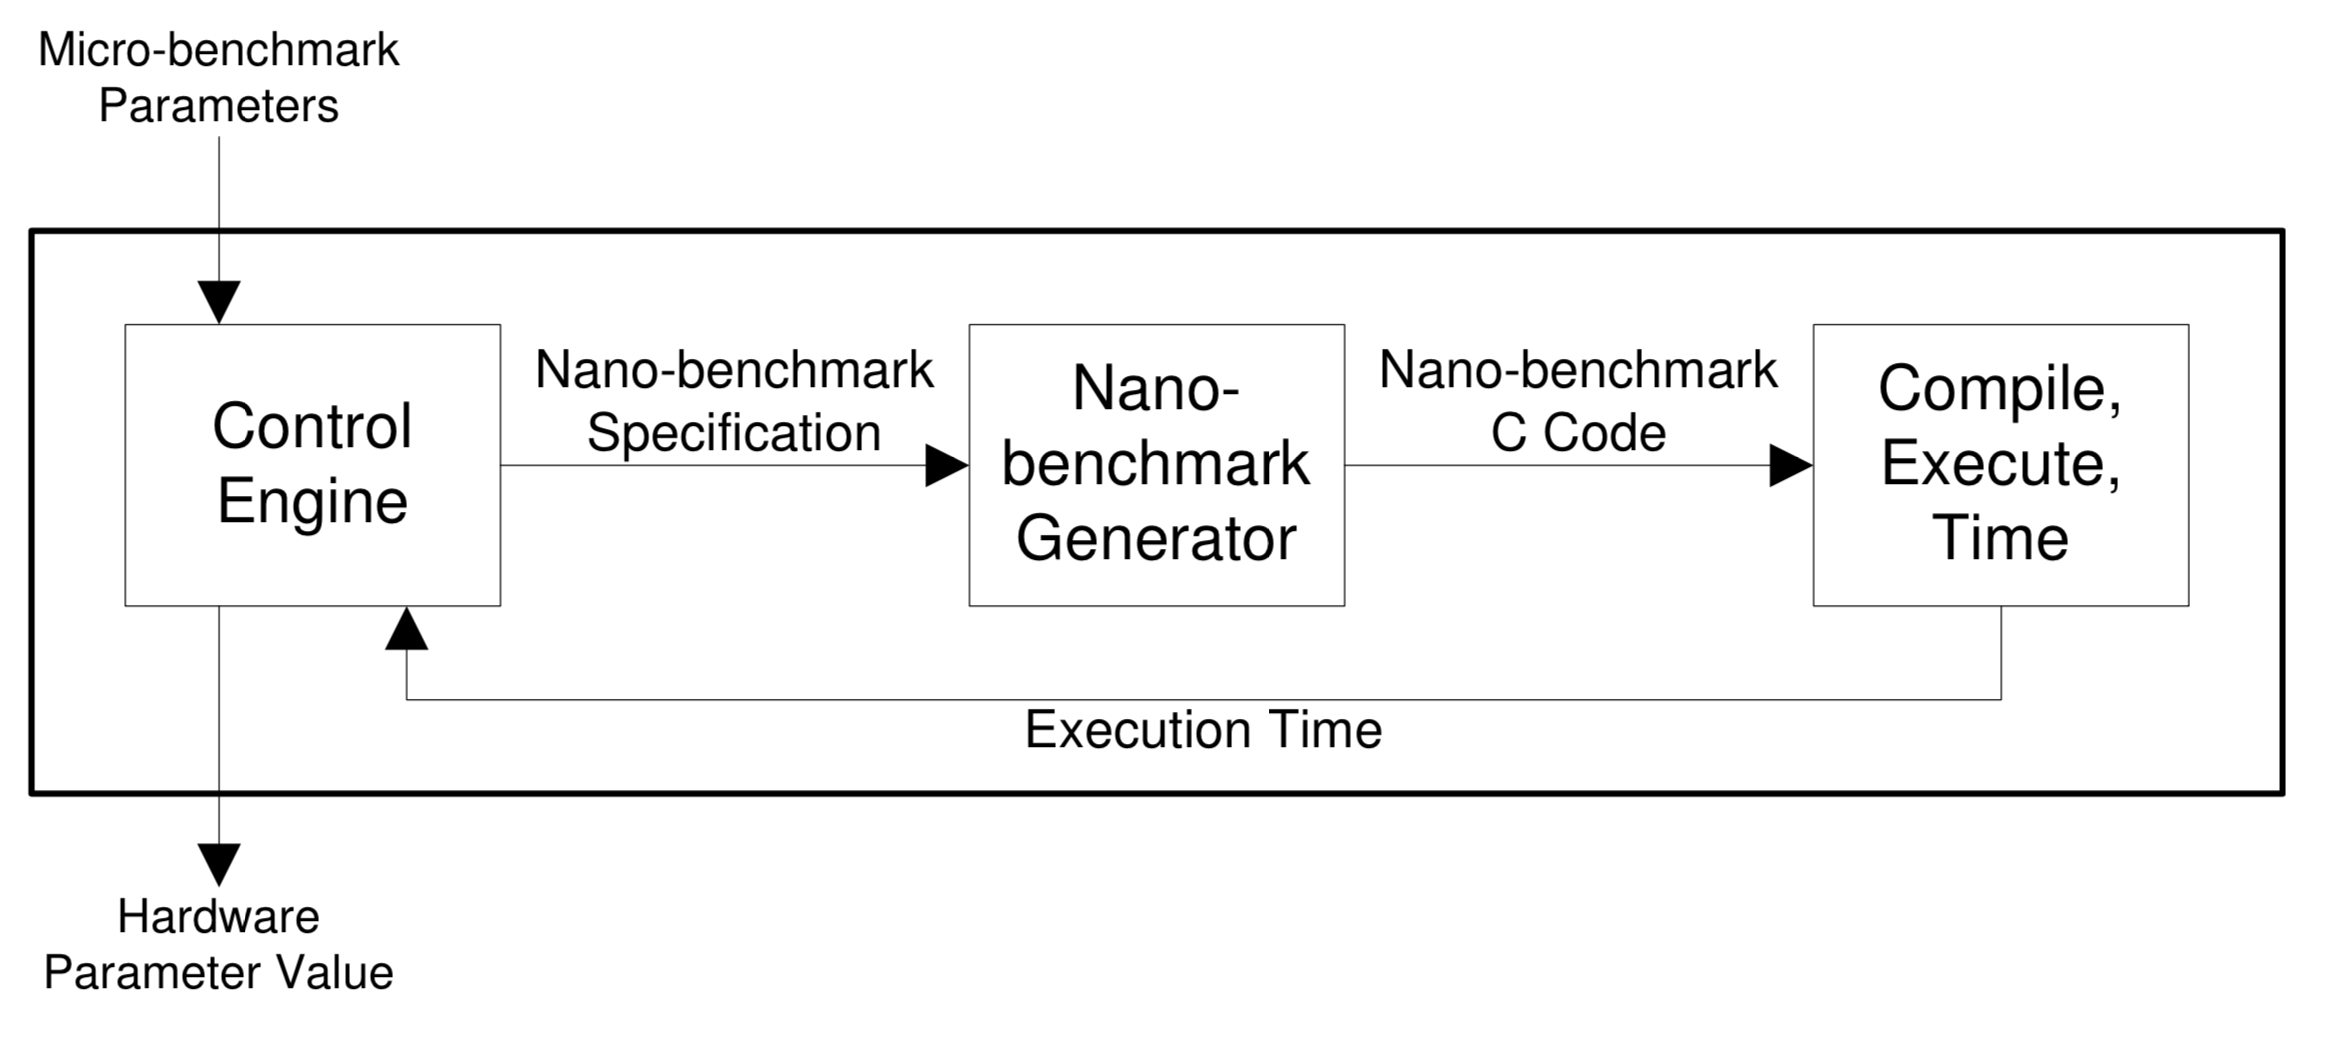
\includegraphics[width=10cm]{images/bench_xray.png}
    \caption{ Structure d'un micro-benchmark réalisé grâce à X-Ray  \cite{Yotov2004}.
    \label{pic_bench_xray}}
\end{figure}


\paragraph{P-Ray \cite{Duchateau2008}.} Dans le but de permettre à certaines librairie (ATLAS, SPIRAL ou FFTW) de s'auto-optimiser P-Ray permet de mesurer certains paramètres matériels. De la même façon que X-Ray et LMbench, l'apport de P-Ray permet de trouver ces spécifications pour des processeurs multi-coeurs. P-Ray permet de décrire la répartition des caches entre les coeurs, la topologie d'interconnexion des processeurs ainsi que les mécanismes de cohérence de caches. Leurs expérimentations montrent des résultats très précis comme la mesure de la latence de communication entre deux coeurs à travers le cache L3, L2 ou entre deux processeurs. Un effort particulier a été apporté pour éviter des optimisations du compilateurs et du prefetcher pouvant altérer les performances mesurées. Le benchmark de P-Ray a hérité d'un problème de X-Ray rendant impossible la portabilité du code entre différent systèmes d'exploitation. L'allocation mémoire suppose que toute les adresses physique soient contigues et cette caractéristiques dépend du système d'exploitation (les pages larges pouvant ne pas être disponibles).
Le code de P-Ray n'est cependant pas libre de droit.

\paragraph{Servet \cite{gonzalez2010servet}.} La suite Servet permet de mesurer certaines caractéristiques matériels telles que la hiérarchie de cache (taille, partage entre les coeurs) ou la bande passante mémoire. Ce travail ajoute a X-Ray et P-Ray des mesures des paramètres d'interconnexion pour la communication d'une mémoire distribuée ainsi qu'une méthodologie et une nouvelle technique de mesure. Une suite de benchmark permet aussi d'évaluer où se formeront les goulots d'étranglements lorsque plusieurs coeurs accèdent à la mémoire centrale. Enfin, Servet mesure la distance entre les coeurs en mesurant la latente de communication permettant à une application de placer plus efficacement les processus sur les différents coeurs.




\paragraph{Likwid}
\textbf{TODO}

Runs in user-space. Uses common kernel interfaces or perf_event
 Counts per HW thread (knowledge about processes)
 Derives metrics out of raw counter values

https://www.tdx.cat/bitstream/handle/10803/666955/TMR1de1.pdf?sequence=1

 A Toolset for performance-oriented developers/users
 Get system topology
 Place threads according system topology (affinity domains)
 Run micro-benchmarks to check system features
 Measure hardware events during application runs
 Determine energy consumption
 Manipulate CPU/Uncore frequencies


The LIKWID tool suite [17] includes the likwid-bench microbenchmarking framework, which provides a set of assembly language kernels. They cover a vari- ety of streaming access schemes. In addition the user can extend the framework by writing new assembly code loop bodies. likwid-bench takes care of loop counting, thread parallelism, thread placement, ccNUMA page placement and performance (and bandwidth) measurement. It does not, however, perform hardware event count- ing. For the HPM measurements we thus use likwid-perfctr, which is also a part of the LIKWID suite. It uses a simple command line interface but provides a comprehensive set of features for the users. Likwid-perfctr supports almost all interesting core and uncore events for the supported CPU types. In order to relieve the user from having to deal with raw event counts, it supports performance groups, which combine often used event sets and corresponding formulas for computing de- rived metrics (e.g., bandwidths or FLOP rates). Moreover, likwid-perfctr pro- vides a Marker API to instrument the source code and restrict measurements to certain code regions. Likwid-bench already includes the calls to the Marker API in order to measure only the compute kernel.





~\\

\subsubsection{Les benchmark mémoire}
%%%%%%%%%%%%%%%%%%%%%%%%%%%%%%%%%


\paragraph{lmbench \cite{HPC:lmbench}} Lmbench is a suite of portable benchmarks used to measure important characteristics of the memory such as bandwidth, memory latency and performance of the different cache levels.

\paragraph{Calibrator}


\paragraph{Saavedra} Ce benchmark est un des plus connus pour caractériser la mémoire. Il utilise une stride fixée pour accéder aux éléments d'un tableau. Le temps nécessaire à ces acces permet de déduire la taille des niveaux de la hiérarchie. Les expérimentations utilise des couples de $\{taille de tableau, taille de stride\}$. La taille du tableau augmente jusqu'à atteindre la taille du cache mesuré. La taille des strides est limitée a des tailles de puissance de 2 et ne dépassera jamais la taille du cache. Le tableau est ainsi parcouru pendant au moins une seconde. Comme le souligne \cite{Yotov2005} le problème d'une telle approche est de vouloir mesurer tout les niveaux de la hiérarchie simultanément. Les mesures peuvent alors être influencées par différents paramètres de différents niveaux de caches. Ces mesures doivent être interprétés par l'utilisateur, le programme ne créant pas automatiquement la hiérarchie. La lecture et l'écriture son réalisés sur la même données pouvant introduire des conflits dans le tampons d'écriture  \cite{Yotov2005}. Le benchmark assume que les donnés sont continues en mémoire mais n'utilise pas de pages larges.


\paragraph{X-ray}
Le travail \cite{Yotov2005} utilise X-Ray pour implémenter des micro-benchmarks pour mesurer la capacité, l'associativité, la taille des blocs ainsi que la latence de chaque niveaux de la hiérarchie de cache ainsi que du TLB. Contrairement aux benchmarks existants, l'outil mesure un niveau à la fois lui permettant d'être plus précis que les approches traditionnelles (X-Ray, Calibrator, lmbench et MOB). Utiliser X-Ray pour implémenter leur benchmark leur permet de mesurer la fréquence du processeur ansi que la latence et le débit instructions. Malheureusement, le code de X-Ray n'a pas été maintenu et n'est plus disponible au téléchargement.


\paragraph{STREAM} Le code STREAM permet de mesurer la bande passante mémoire atteignable grâce à l'implémentation de quatre noyaux: COPY ($c=a$), SCALE ($b=\alpha \times c$), ADD ($c=a+b$) et TRIAD ($a=b+\alpha \times c$).


The second worldwide known benchmark is STREAM \cite{HPC:stream} that was originally developed to understand the performance differences between two architectures for a weather application.

The main problem with those benchmarks comes from their artificial code not representing real application. To this end, other specific benchmarks have been developed to reflect how real application would perform. On recent HPC architectures, having a good HPL performance is no longer correlated with having good performance with real applications, so the HPCG was introduced \cite{HPC:hpcg}. 

\paragraph{HPCG} This benchmark fills the gap by implementing some micro-benchmarks more representative of the workload used in the industry as sparse matrix-vector multiplication or sparse triangular solvers.